\section*{Bedienungsanleitung}
\subsection*{Auswählen von Dateien}
Um Dateien Auswählen zu können, muss im Hauptbereich auf File \textrightarrow change Files... gedrückt werden. Es öffnet sich ein neues Fenster. In diesem können Bilder, Ordner oder eine Datenbank ausgewählt werden. Ordner auswählen wird empfohlen, wenn viele Unterordner genutzt werden, oder die Ausgewählten Bilder eine Anzahl von 50.000 überschreitet. Die Ordnerstruktur wird im rechten Bereich dargestellt, wobei alle Oberordner, welche keine Ausgewählten Bilder beinhalten. Ein Ordner und all seine Unterordner, können gelöscht werden. Beim Verlassen des Fensters werden die Änderungen nur dann übernommen, wenn auf Speichern  gedrückt wird.
\begin{figure}[h]
    \centering
    \subfloat[\centering Dateibereich öffnen]{
        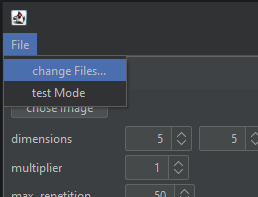
\includegraphics[height=5cm]{images/Bedienungsanleitung/change Files.png}
        \label{change Files}
    }
    \subfloat[\centering Dateiein Auswählen]{
        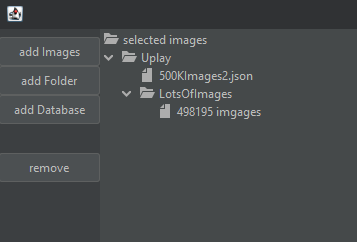
\includegraphics[height=5cm]{images/Bedienungsanleitung/change Files UI.png}
        \label{change Files UI}
    }
    \captionof{Ausschnitt}{Dateien Auswählen}
    \label{Dateien Auswählen}
\end{figure}

\newpage
\subsection*{Vorbereiten eines Render-Auftrages}
Um einen Auftrag vorzubereiten, kann man ein Grundbild auswählen. Die Spalten auf X und Y Ebene kann unter dem Bereich ``Dimensions'' angepasst werden. Es wird im Bildbereich auf der rechten Seite ein Netz aus Linien angezeigt, welche die Größe der Sektoren darstellt. Im Bereich ``multiplier'' kann angegeben werden, um welchen Faktor das Endbild skaliert werden soll. Es werden nur ganze Zahlen akzeptiert. Der Bereich ``max. repetition'' gibt an, wie häufig ein einzelnes Bild verwendet werden darf. Die Qualität von der Berechnung der durchschnittlichen Farbe und der Skalierung kann in einem Dropdown Menü ausgewählt werden.\\ Der Auftrag kann abgeschickt werden, oder alternativ auch eine Datenbank mit der ausgewählten Quantität erstellt werden kann.
\begin{figure}[h]
    \centering
    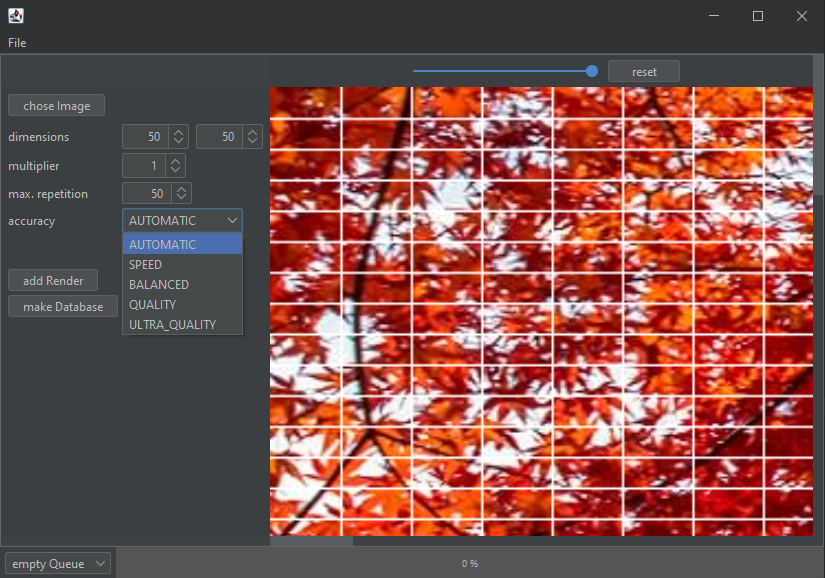
\includegraphics[height=9cm]{images/Bedienungsanleitung/normal UI.png}
    \captionof{Ausschnitt}{Hauptbereich}
    \label{Hauptbereich}
\end{figure}
Es können auch mehre Aufträge abgeschickt werden. Es wird jedoch nur einer bearbeitet. Zusätzlich wird der aktuelle Progress angegeben.
\begin{figure}[h]
    \centering
    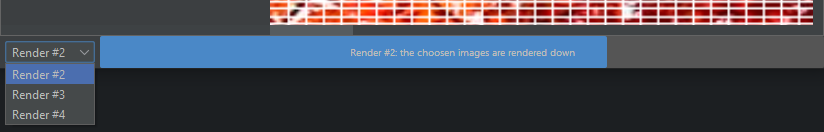
\includegraphics[height=2cm]{images/Bedienungsanleitung/render queue.png}
\end{figure}

\newpage
\subsection*{Bearbeiten des Fertigen Bildes}
Ist der Auftrag abgeschlossen, öffnet sich das fertige Bild in einem neuen Fenster. In diesem kann das Bild vor dem speichern noch bearbeitet werden. Das original Bild kann mithilfe eines Schieberegler mit unterschiedlicher Transparenz auf das Bild gelegt werden.
\begin{figure}[h]
    \centering
    \subfloat[\centering ohne Transparenz]{
        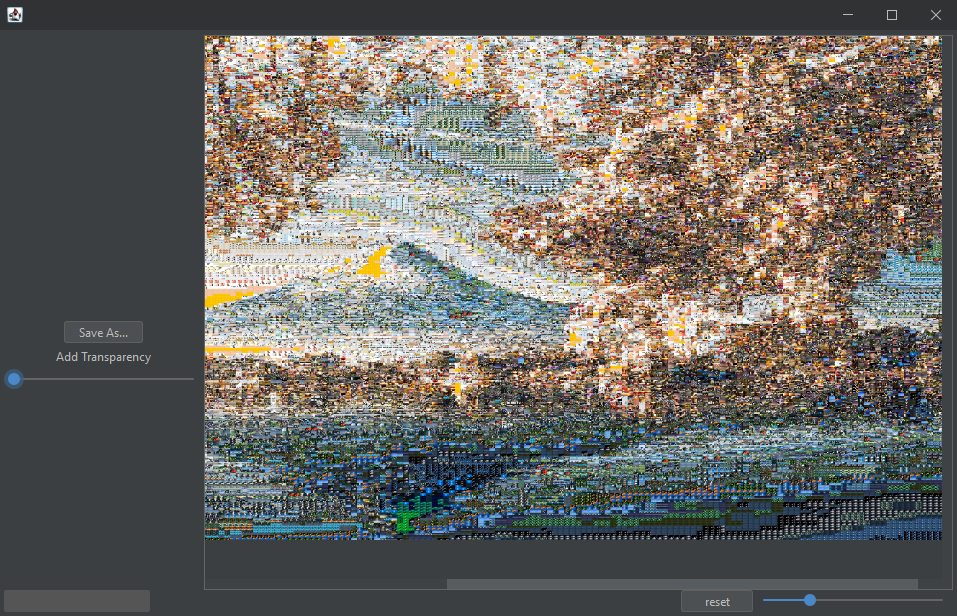
\includegraphics[height=4cm]{images/Bedienungsanleitung/finished Picture.png}
        \label{fertig ohne}
    }
    \subfloat[\centering mit Transparenz]{
        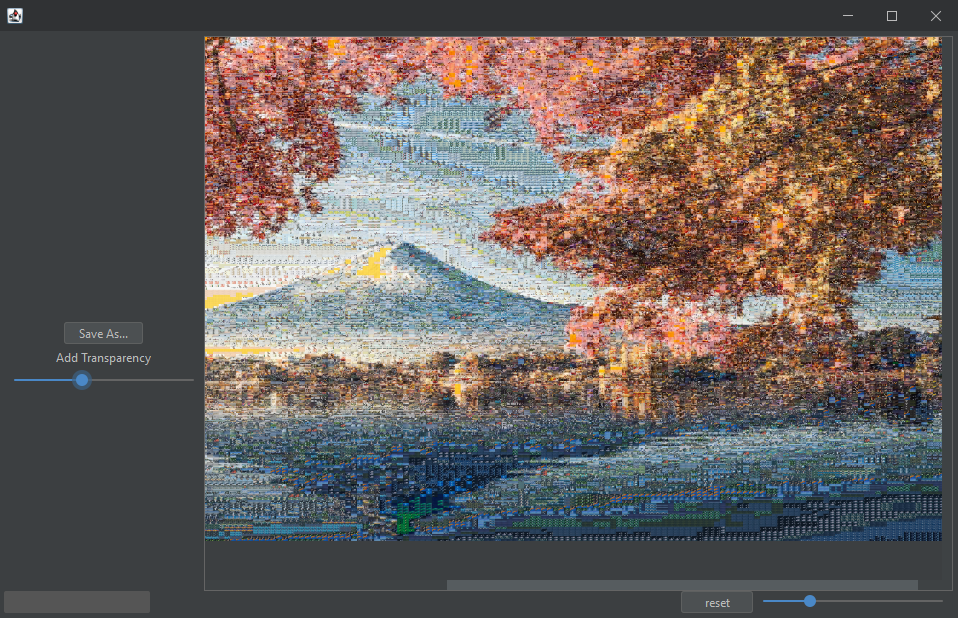
\includegraphics[height=4cm]{images/Bedienungsanleitung/finished Picture transparency.png}
        \label{fertig mit}
    }
    \captionof{Ausschnitt}{Bildbearbeitung}
    \label{fertig}
\end{figure}

\subsection*{Nutzung des Testbereich}
Der Testbereich kann aus dem Hauptbereich erreicht werden, wenn in dem Menü auf Files \textrightarrow test Mode geklickt wird. Es wird sich ein neues Fenster öffnen. In dem Fenster kann zwischen den unterschiedlichen Test Modi ausgewählt werden. Auch können spezifische Einstellungen vorgenommen werden. Dabei kann man auswählen aus welcher Quelle die verwendeten Bilder generiert werden. Zur Auswahl stehen generierte Bilder und Bilder, welche aus dem Internet heruntergeladen werden. Die Wiederholrate der Tests kann auch spezifiziert werden. Bei jeder Wiederholung wird die Anzahl der Bilder erhöht. Die Anzahl an Bildern kann im rechten Feld eingegeben werden. Außerdem gibt es die Möglichkeit den Test aufzuzeichnen. Ein bereits laufender Test kann abgebrochen werden. Dies ist aber als Not-Maßnahme gedacht. Es wird empfohlen das Programm danach neu zu starten.

\begin{figure}[h]
    \centering
    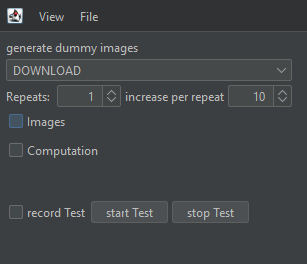
\includegraphics[height=4.5cm]{images/Bedienungsanleitung/test Mode UI.png}
    \captionof{Ausschnitt}{Testbereich}
    \label{Testbereich}
\end{figure}

Die Unterschiedlichen Test Szenarien sind: Die durchschnittliche Farbe berechnen, eine Datenbank erstellen, Bilder skalieren und die besten Bilder berechnen. In dem Bilder Sektor, werden alle nötigen Einstellungen angezeigt. Diese variieren nach Auswahl.

\begin{figure}[h]
    \centering
    \subfloat[\centering Bilder]{
        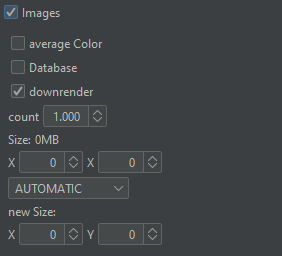
\includegraphics[height=6cm]{images/Bedienungsanleitung/test mode Images.png}
        \label{Test_Bilder}    
    }
    \subfloat[\centering Berechnung]{
        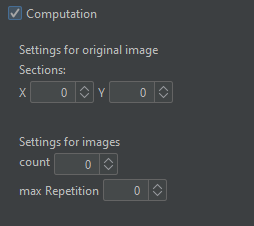
\includegraphics[height=6cm]{images/Bedienungsanleitung/test mode Computation.png}
        \label{Test_Berechnung}
    }
    \captionof{Ausschnitt}{Test Einstellungen}
    \label{Einstellungen}
\end{figure}

Wurde ein Test durchgeführt, so können seine Ergebnisse angesehen werden. Dazu muss auf view \textrightarrow select view \textrightarrow graph gegangen werden. Es erscheinen auf der linken Seite zwei Bereiche. Im oberen stehen alle gemachten Tests. Im unteren Bereich stehen alle Tests, die man ansehen möchte. Um einen Test anzusehen, muss dieser einfach von oben nach unten mit gedrückter Maus gezogen werden.

\begin{figure}[h]
    \centering
    \subfloat[\centering Tests auswählen]{
        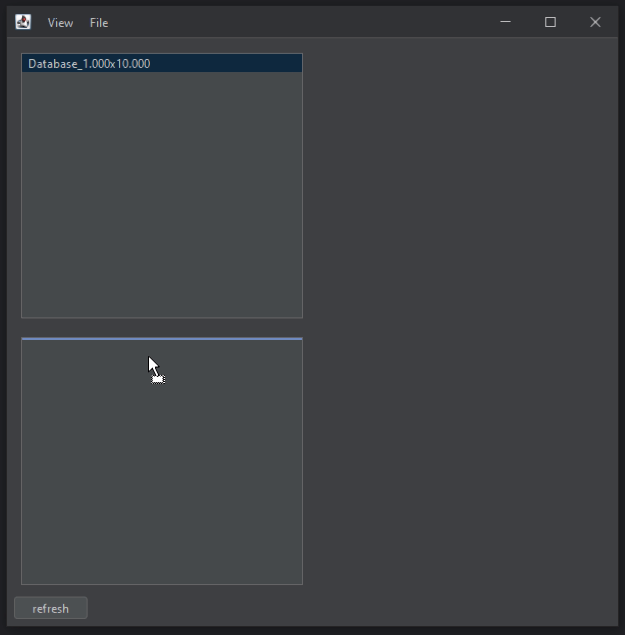
\includegraphics[height=8cm, valign=c]{images/Bedienungsanleitung/test mode viewer.png}
    }
    \subfloat[\centering Graph betrachten]{
        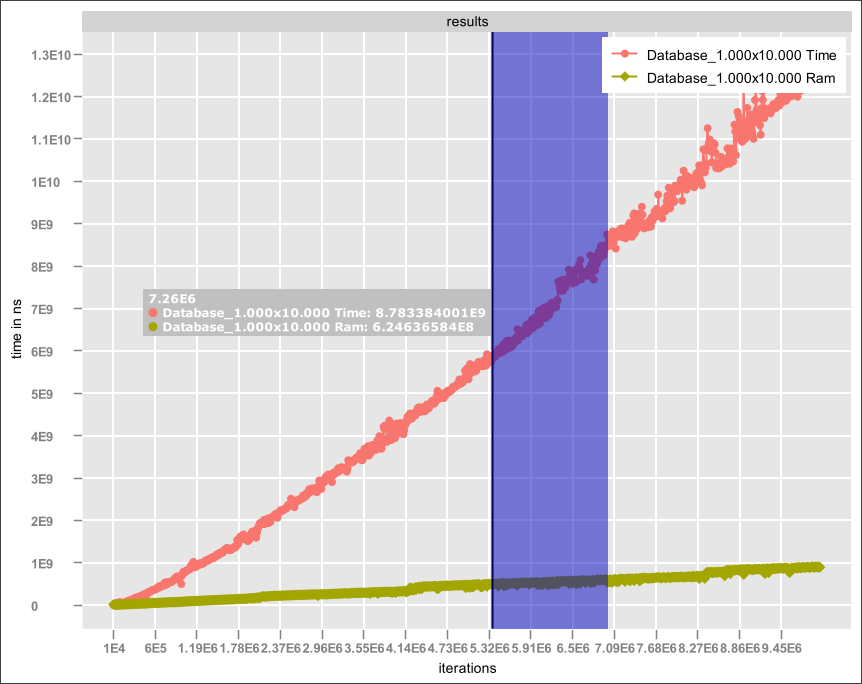
\includegraphics[height=4cm, valign=c]{images/Bedienungsanleitung/Test Graph.png}
        \vphantom{\includegraphics[height=7.7cm, width=0.1cm, valign=c]{example-image-a}}
    }
    \captionof{Ausschnitt}{Tests ansehen}
    \label{Tests auswählen}
\end{figure}